\section{Introduction}

Perhaps you killed someone, perhaps you were the most horrible criminal in the country for stealing cows and selling them over coast, or perhaps you were a peasant who found out that a prince just went missing, whose appearances were strikingly similar to yours. In old times, all these were valid motives to disappear from the community, and reappear sometime later with another name, another haircut, another identity.

It was also quiet easy to tell lies, and gossip. The only way you could verify someone's story, was to ask around, and believe your most trustworthy person, like your sister or brother. However, as the saying goes, ``lies have short legs''. Stories could only travel as fast as the fastest camel, or horse, and as far as what your kingdom allowed you to. Because of this, news spreading was slow, and mostly unreliable, as the person carrying the news would most likely alter it, forget it or change it completely.

In fact, before modern identification, the only way you could prove who you were and if what you were saying was true, was your word.

Today, disappearing is not as simple as the old times. But lies just got longer legs. So long, that they can reach not only your hateful neighbor or the ears of your handsome Queen, but overseas, on a small island in the Pacific Ocean with an internet antenna, onto the screen of your Twitter follower ``Leila31XoXo''.

In the following chapters we will explore what ``lies'' beneath fake profiles, generated profile pictures and their impact on modern society.

\begin{figure}
    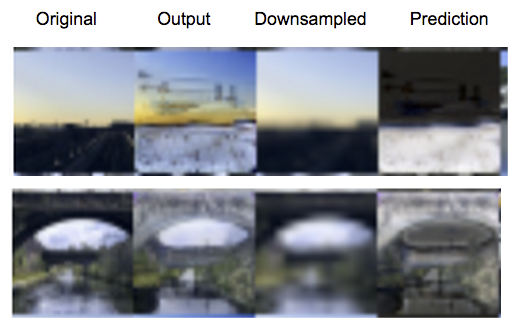
\includegraphics[width=\linewidth]{00_Introduction/eyescream_predicted16.png}
    \Description[Skyline and bridges, generated by Eyescream (2015)]{Skyline and bridges, generated by Eyescream (2015)}
    \caption{Skyline and bridges, generated by Eyescream (2015)}
    \label{fig:eyescream}
\end{figure}

\begin{figure}
    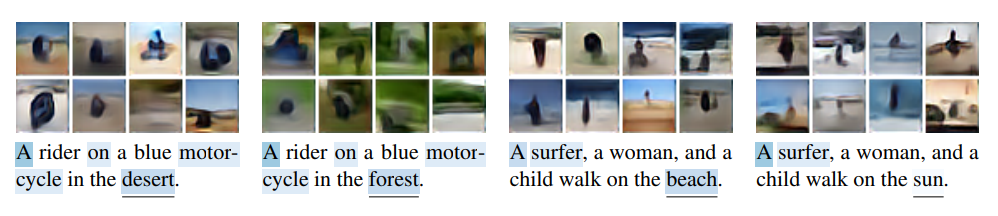
\includegraphics[width=\linewidth]{00_Introduction/gen_from_captions.png}
    \Description[Example of most attended words while changing the background in the caption]{Example of most attended words while changing the background}
    \caption{Example of most attended words while changing the background}
    \label{fig:gen_attention}
\end{figure}
